% !TeX TXS-program:compile = txs:///lualatex

\documentclass[a4paper,11pt]{article}
\usepackage[breakable]{cp-base}
\graphicspath{{./graphics/}}
%variables
\donnees[%
	typedoc=CHAPITRE~,numdoc=6,classe=1\up{ère} 2M2,matiere={[SPÉ.MATHS]}
]

%formatage
\author{Pierquet}
\title{\nomfichier}
\hypersetup{pdfauthor={Pierquet},pdftitle={\nomfichier},allbordercolors=white,pdfborder=0 0 0,pdfstartview=FitH}
%divers
\lhead{\entete{\matiere}}
\chead{\entete{\lycee}}
\rhead{\entete{\classe{} - Chapitre \thepart}}
\lfoot{\pied{\matiere}}
\cfoot{\logolycee{}}
\rfoot{\pied{\numeropagetot}}
\usepackage{setspace}

\begin{document}

\pagestyle{fancy}

\part{CH06 - Trigonométrie}

\section{Mesure d'angle en radians}

\subsection{Le cercle trigonométrique}

\begin{cdefi}
Dans un repère orthonormé $\Rij$, le \textbf{cercle trigonométrique} est le cercle \emph{orienté} de centre $O$, de rayon 1 et parcouru dans le \emph{sens inverse des aiguilles d'une montre}.
\end{cdefi}

\begin{cillustr}
\vspace{-0.2cm}
\begin{center}
	\tikzset{cross/.style={%
			cross out,draw=black,minimum size=2*(#1-\pgflinewidth),inner sep=0pt,outer sep=0pt},%
			cross/.default={1pt}}
	\begin{tikzpicture}[x=1.25cm,y=1.25cm,line width=1.25pt]
		\draw[->,>=stealth] (-1.15,0) -- (3,0) ; \draw[->,>=stealth] (0,-1.15) -- (0,1.75) ;
		\draw[blue] (0,0) circle[radius=1] ;
		\draw[blue] (135:1.2) node {\footnotesize \sf (C)};
		\draw[line width=1pt] (1,0) node[cross=3pt,black]{};
		\draw (0,1) node[above left=0pt] {\footnotesize \sf J} (1,0) node[above right=0pt] {\footnotesize \sf 1} (1,0) node[below right=0pt] {\footnotesize \sf I} ;
		\draw (2,0) node[above] {\tiny \sf axe des abscisses} ;
		\draw[ForestGreen,->,>=stealth] (25:1.5) arc (25:65:1.5) ;
		\draw[ForestGreen] (45:1.65) node {\small \sf +};
	\end{tikzpicture}
\end{center}
\end{cillustr}

\begin{crmq}
Le sens de parcours sur le cercle trigonométrique s'appelle le sens \emph{direct}, le sens \emph{trigonométrique} ou encore sens \emph{positif}.
\end{crmq}

\subsection{Longueur d'arc et mesure en radian}

\begin{cprop}
Si $I$ est le point de coordonnées $(1\,;\,0)$ et $M$ est un point du cercle trigonométrique, alors la longueur de l'arc $\overparen{IM}$ (exprimée dans l'unité de longueur du repère) est proportionnelle à la mesure de l'angle $\widehat{IOM}$.
\end{cprop}

\begin{cdefi}
La \textbf{mesure en radians} d'un angle est égale à la \textbf{longueur de l'arc} qu'il intercepte sur le cercle trigonométrique.
\end{cdefi}

\begin{cillustr}
\vspace{-0.2cm}
\begin{center}
	\tunits{1.25}{1.25}
	\tdefgrille{-1.15}{3}{1}{1}{-1.15}{1.5}{1}{1}
	\begin{tikzpicture}[x=\xunit cm,y=\yunit cm,line width=1.25pt]
		\draw[ForestGreen,fill=ForestGreen!50,opacity=0.5] (0,0) -- (0.48,0) arc (0:130:0.48) -- cycle ;
		\axestikz*[typefleche=stealth] ;
		\axextikz[size=\footnotesize]{-1,1,2} ;
		\axeytikz[size=\footnotesize]{-1,1} ;
		\draw (0,0) node[below left] {\footnotesize $0$} ;
		\draw[darkgray] (0,0) node[above right] {\small \sf O} (1,0) node[above right] {\small \sf I} (130:1) node[above] {\small \sf M} ;
		\draw[blue] (0,0) circle[radius=1] ; \draw (0,0) -- (130:1) ;
		\draw[red,line width=1.5pt] (1,0) arc (0:130:1) ;
		\foreach \Point in {(0,0),(1,0),(130:1)} \draw[line width=0.75pt,darkgray,fill=gray] \Point circle[radius=2pt] ;
		\draw[ForestGreen] (0.20,0.6) node {\tiny \sf Angle de $\mathsf{\theta}$ radians};
		\draw[red] (65:1.05) node[right] {\tiny \sf Arc de $\mathsf{\theta}$ unités de longueur};
	\end{tikzpicture}
\end{center}
\end{cillustr}

\begin{crmq}[ - Exemple]
Les mesures en radians ou en degrés sont donc proportionnelles. Un angle de $\pi$ radians mesure 180\ensuremath{^\circ} donc une simple règle de proportionnalité permet de convertir d'une unité à l'autre : {\footnotesize \begin{tabularx}{1.5cm}{Y|Y} 180&$\pi$ \\ \hline $d$&$r$ \end{tabularx}}.

Par exemple, $90\ensuremath{^\circ} = \dfrac{\pi}{2}$ rad  ; $\frac{2\pi}{3} \text{rad} =  120 \ensuremath{^\circ}$.
\end{crmq}

\section{Enroulement autour du cercle}

\subsection{Le principe}

\begin{cdefi}
Dans un repère orthonormé $\Rij$, on considère le cercle trigonométrique $\mathscr{C}$ ; le point $I$ de coordonnées $(1\,;\,0)$ et  la tangente $\mathscr{D}$ à $\mathscr{C}$ en $I$. On gradue la droite $\mathscr{D}$ en choisissant comme origine le point d'accroche $I$ (l'unité étant celle du repère).

En \emph{enroulant} cette droite $\mathscr{D}$ autour du cercle, on va pouvoir \og graduer \fg{}  $\mathscr{C}$ :
\begin{itemize}
	\item à chaque graduation $x$ de la droite va correspondre un et un seul point $M$ sur le cercle, appelé \textbf{point image} de $x$ ;
	\item inversement, tout point $M$ du cercle va être l'image d'une \emph{infinité} de graduations de la droite, puisqu'on pourra avoir fait plusieurs tours avant de se \og poser \fg{} sur le point $M$.
\end{itemize}
\end{cdefi}

\begin{cillustr}
\vspace{-0.2cm}
\begin{center}
	\tunits{1.75}{1.75}
	\tdefgrille{-2.25}{2.25}{1}{1}{-3.25}{1.95}{1}{1}
	\begin{tikzpicture}[x=\xunit cm,y=\yunit cm,line width=1.25pt]
		%COORDONNÉES
		\coordinate (A) at (0.8030891985946332,0.9489560907235874) ;
		\coordinate (B) at (-0.038218144126171916,1.4467133524906286) ;
		\coordinate (C) at (-1.0079914833239498,1.2770337234951197) ;
		\coordinate (D) at (-1.696143627182363,0.5689538121942858) ;
		\coordinate (E) at (-1.8960096583336494,-0.4018233394326452) ;
		\coordinate (F) at (-1.584471132921636,-1.3419867475443141) ;
		\coordinate (G) at (-0.8609551506944302,-2.032442621128445) ;
		\coordinate (H) at (0.09151065412969567,-2.3286691570259115) ;
		\coordinate (I) at (1.0781855073536135,-2.196903154121031) ;
		\coordinate (J) at (1.9310796896114646,-1.678963054543094) ;
		%SUITE
		\tgrilles[thin,dashed,lightgray] ;
		\axestikz*[typefleche=stealth] ;
		\axextikz[size=\footnotesize]{-2,-1,1,2} ; \axeytikz[size=\footnotesize]{-3,-2,-1,1} ;
		\draw (0,0) node[above left] {\footnotesize \sf O} ;
		\draw (1,0) node[above right] {\footnotesize \sf I} ;
		\draw[purple] (1,-3.25) -- (1,0) ;
		\draw[blue] (0,0) circle[radius=1] ;
		\foreach \y in {-3,-2,-1} \draw[purple] ($(1,\y)+(-4pt,0)$) -- ($(1,\y)+(4pt,0)$) node[purple,right] {\footnotesize $\mathsf{\y}$};
		\clip (\xmin,\ymin) rectangle (\xmax,\ymax) ;
		\draw[domain=0:6,samples=500,ForestGreen] plot ({deg(\x)}:{0.28*\x+1});
		%enroulement
		\foreach \Node/\Angle in {A/57.295,B/114.592,C/171.887,D/229.183}
			\draw[densely dashed,ForestGreen] (\Node) to[bend right] (\Angle:1) ;
		\draw[densely dashed,ForestGreen] (E) to[bend right=40] (286.479:1) ;
		\draw[densely dashed,ForestGreen] (F) to[bend right=60] (343.775:1) ;
		%points sur objets
		\foreach \Angle in {0,57.295,90,114.592,171.887,180,229.183,270,286.479,343.775} \draw[line width=0.75pt,darkgray,fill=blue!50] (\Angle:1) circle[radius=2pt] ;
		\foreach \Node/\Valeur/\Pos in {A/1/above right,B/2/above left,C/3/above left,D/4/above left,E/5/left,F/6/below left,G/7/below left,H/8/below right,I/9/below right,J/10/below right} \draw[line width=0.75pt,black,fill=ForestGreen] (\Node) circle[radius=2.5pt] node[\Pos,ForestGreen] {\footnotesize $\mathsf{\Valeur}$} ;
	\end{tikzpicture}
\end{center}
\end{cillustr}

\begin{crmq}
La demi-droite graduée négativement s'enroule dans le sens contraire autour du cercle.
\end{crmq}

\begin{cprop}
Si deux graduations de la droite ont le même point-image sur le cercle, alors elles diffèrent d'un nombre entier de tours. Autrement dit, si $x$ et $y$ ont le même point-image, alors : \[y=x+k\times 2\pi \text{ où } k \text{ est un nombre entier.}\]%
On dit que $x$ et $y$ sont égaux \emph{à $2\pi$ près} ou égaux \emph{modulo $2\pi$} ou congrus \emph{modulo $2\pi$}.
\end{cprop}

\begin{ccscq}
On appelle \textbf{mesure principale} d'un angle $x$ l'unique l'angle $y$ tel que $\begin{dcases} y=x+k\times 2\pi \\ -\pi < y \pp \pi \end{dcases}$.

On peut déterminer la mesure principale par \og réductions \fg{} de $2\pi$ (on \og rajoute \fg{} ou on \og enlève \fg{} des tours).
\end{ccscq}

\subsection{Valeurs remarquables}

\begin{crmq}
Dans la mesure où le périmètre du cercle est $2\pi$, les graduations entières de la droite ne se poseront pas sur des points particuliers du cercle. Il est plus judicieux de graduer la droite avec des fractions et des multiples de $\pi$, ces valeurs ayant des points-images plus faciles à placer sur le cercle !
\end{crmq}

\begin{cprop}
Les valeurs remarquables sur le cerlce trigo sont les valeurs $0\,;\,\frac{\pi}{6}\,;\,\frac{\pi}{4}\,;\,\frac{\pi}{3}\,;\,\frac{\pi}{2}$ et toutes les valeurs associées dans les autres quadrants du cercle.

\smallskip

Pour les placer facilement sur le cercle, il suffit de \og découper \fg{} le demi-cercle supérieur de longueur $\pi$ en 6 ; 4 ; 3 ou 2.
\end{cprop}

\begin{cexercice}
Placer ces valeurs remarquables sur le premier quadrant du cercle ci-dessous, puis placer sur le cercle les valeurs associées dans les autres quadrants (en fonction du \og sens de parcours \fg) :
\begin{center}
	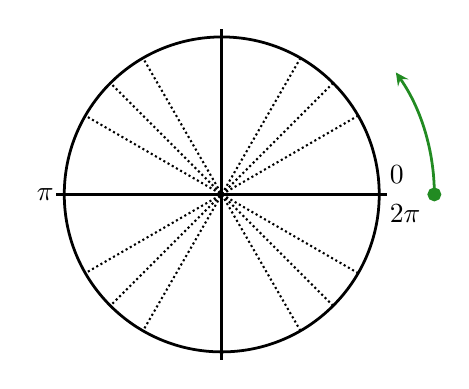
\begin{tikzpicture}[x=2cm,y=2cm,line width=1pt]
		\draw (-1.05,0) -- (1.05,0) (0,-1.05) -- (0,1.05) ;
		\draw (0,0) circle[radius=1] ;
		\foreach \angle in {-60,-45,-30,30,45,60} \draw[densely dotted,line width=0.75pt] (\angle:1) -- ({\angle+180}:1) ;
		\draw (1,0) node[above right] {$0$} (1,0) node[below right] {$2\pi$} (-1,0) node[left] {$\pi$} ;
		\draw[ForestGreen,->,>=stealth] (0:1.35) arc (0:35:1.35) ;
		\filldraw[ForestGreen] (1.35,0) circle[radius=2pt] ;
	\end{tikzpicture}
	\hspace{2cm}
	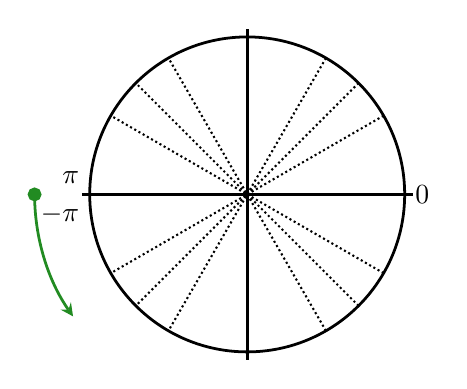
\begin{tikzpicture}[x=2cm,y=2cm,line width=1pt]
		\draw (-1.05,0) -- (1.05,0) (0,-1.05) -- (0,1.05) ;
		\draw (0,0) circle[radius=1] ;
		\foreach \angle in {-60,-45,-30,30,45,60} \draw[densely dotted,line width=0.75pt] (\angle:1) -- ({\angle+180}:1) ;
		\draw (1,0) node[right] {$0$} (-1,0) node[below left] {$-\pi$} (-1,0) node[above left] {$\pi$} ;
		\draw[ForestGreen,->,>=stealth] (180:1.35) arc (180:215:1.35) ;
		\filldraw[ForestGreen] (-1.35,0) circle[radius=2pt] ;
	\end{tikzpicture}
\end{center}
\end{cexercice}

\section{Fonctions sinus et cosinus}

\subsection{Définition}

\begin{cdefi}
Soit $x$ un nombre réel et $M$ son point-image sur le cercle trigonométrique. Par définition :
\begin{itemize}
	\item l'\textbf{abscisse} de $M$ est appelée le \textbf{cosinus} de $x$, noté $\cos(x)$ ;
	\item l'\textbf{ordonnée} de $M$ est appelée le \textbf{sinus} de $x$, noté $\sin(x)$.
\end{itemize}
Le point $M$ a donc pour coordonnées $\big(\cos(x)\,;\,\sin(x)\big)$.
\end{cdefi}

\begin{cillustr}
\vspace{-0.2cm}
\begin{center}
	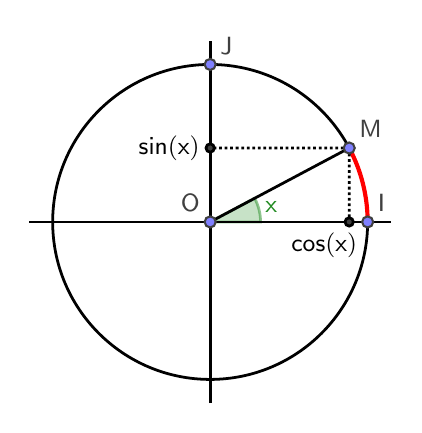
\begin{tikzpicture}[x=2cm,y=2cm,line width=1pt]
		\draw[ForestGreen,fill=ForestGreen!50,opacity=0.5] (0,0) -- (0.32,0) arc (0:28:0.32) -- cycle ;
		\draw (-1.15,0) -- (1.15,0) (0,-1.15) -- (0,1.15) ;
		\draw (0,0) circle[radius=1] ;
		\draw (0,0) -- (28:1) ;
		\draw[red,line width=1.5pt] (1,0) arc (0:28:1) ;
		\draw[densely dotted] (28:1) -- (0.8829,0) ;
		\draw[densely dotted] (28:1) -- (0,0.4695) ;
		\foreach \Point/\Nom/\Pos in {(0,0)/O/above left,(1,0)/I/above right,(0,1)/J/above right,(28:1)/M/above right} \draw[line width=0.75pt,darkgray,fill=blue!50] \Point circle[radius=2pt] node[darkgray,\Pos] {\small \sf \Nom} ;
		\draw[black,fill=darkgray] (0.8829,0) circle[radius=1.5pt] (0,0.4695) circle[radius=1.5pt] ;
		\draw (1,0) node[below left] {\small $\mathsf{cos(x)}$} ;
		\draw (0,0.4695) node[left] {\small $\mathsf{sin(x)}$} ;
		\draw[ForestGreen] (14:0.4) node {\small $\mathsf{x}$} ;
	\end{tikzpicture}
\end{center}
\end{cillustr}

\begin{cprop}[ : lien avec les formules \og SOHCAHTOA \fg]
Ces définitions sont cohérentes avec celles vues au collège, dans un triangle rectangle !
\end{cprop}

\begin{cdemoblanc}
En effet, choisissons un réel $x$ dans le premier quadrant.

Soit $H$ le projeté orthogonal de $M$ sur l'axe des abscisses : le triangle $OHM$ est rectangle en $H$. On peut donc appliquer les formules classiques : \[\sin(x)=\frac{\mbox{côté opposé}}{\mbox{hypoténuse}}=\frac{HM}{OM}  \text{ et } \cos(x)=\frac{\mbox{côté adjacent}}{\mbox{hypoténuse}}=\frac{OH}{OM}. \]%
Comme le cercle est le cercle trigonométrique, son rayon est égal à 1 donc $OM=1$. On obtient donc bien : \[\sin(x)=HM=\mbox{ordonnée de }M \text{ et } \cos(x)=OH=\mbox{abscisse de }M. \]%
Cette nouvelle définition permet d'étendre les notions de cosinus et sinus à des angles obtus, ou négatifs.
\vspace{-0.2cm}
\begin{center}
	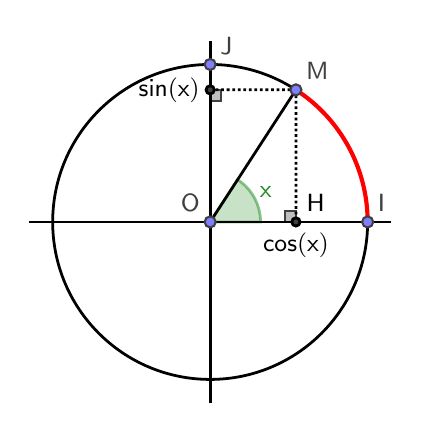
\begin{tikzpicture}[x=2cm,y=2cm,line width=1pt]
		\draw[ForestGreen,fill=ForestGreen!50,opacity=0.5] (0,0) -- (0.32,0) arc (0:57:0.32) -- cycle ;
		\draw[line width=0.75pt,darkgray,fill=lightgray] (0.5446,0) rectangle ++(-4pt,4pt) ;
		\draw[line width=0.75pt,darkgray,fill=lightgray] (0,0.8387) rectangle ++(4pt,-4pt) ;
		\draw (-1.15,0) -- (1.15,0) (0,-1.15) -- (0,1.15) ;
		\draw (0,0) circle[radius=1] ;
		\draw (0,0) -- (57:1) ;
		\draw[red,line width=1.5pt] (1,0) arc (0:57:1) ;
		\draw[densely dotted] (57:1) -- (0.5446,0) ;
		\draw[densely dotted] (57:1) -- (0,0.8387) ;
		\foreach \Point/\Nom/\Pos in {(0,0)/O/above left,(1,0)/I/above right,(0,1)/J/above right,(57:1)/M/above right} \draw[line width=0.75pt,darkgray,fill=blue!50] \Point circle[radius=2pt] node[darkgray,\Pos] {\small \sf \Nom} ;
		\draw[black,fill=darkgray] (0.5446,0) circle[radius=1.5pt] (0,0.8387) circle[radius=1.5pt] ;
		\draw (0.5446,0) node[below] {\small $\mathsf{cos(x)}$} ;
		\draw (0.5446,0) node[above right] {\small \sf H} ;
		\draw (0,0.8387) node[left] {\small $\mathsf{sin(x)}$} ;
		\draw[ForestGreen] (28:0.4) node {\small $\mathsf{x}$} ;
	\end{tikzpicture}
\end{center}
\end{cdemoblanc}

\begin{crmq}
On a ainsi décrit un mécanisme qui, à tout réel $x$ fait correspondre une et une seule valeur de $\cos(x)$. On a donc défini une \emph{fonction}, qu'on appelle la fonction \emph{cosinus}. Même chose pour la fonction \emph{sinus}.
\end{crmq}

\subsection{Valeurs remarquables}

\begin{cprop}[ : tableau de valeurs]
Les valeurs exactes des cosinus et sinus des valeurs remarquables sur le cercle trigonométrique sont à \textbf{connaître}. Il suffit de retenir celles du premier quadrant, les autres se retrouvent par symétrie et changement de signes.

\renewcommand{\arraystretch}{2.5}
\begin{center}
	\begin{tabularx}{10cm}{|c|Y|Y|Y|Y|Y|}
		\hline
		angle (en radians) & $0$ & $\frac{\pi}{6}$ & $\frac{\pi}{4}$ & $\frac{\pi}{3}$ & $\frac{\pi}{2}$ \\ 
		\hline
		cosinus & $1$ & $\frac{\sqrt{3}}{2}$ & $\frac{\sqrt{2}}{2}$ & $\frac{1}{2}$ & 0 \\ 
		\hline
		sinus & $0$ & $\frac{1}{2}$ & $\frac{\sqrt{2}}{2}$ & $\frac{\sqrt{3}}{2}$ & 1 \\ 
		\hline
	\end{tabularx}
\end{center}
\end{cprop}

\begin{crmq}
Le cercle trigonométrique \textit{transparent} permet de lire directement les valeurs particulières des angles \og classiques \fg.
\end{crmq}

%\begin{cdemoblanc}
%Voir exercices.
%\end{cdemoblanc}

\subsection{Propriétés complémentaires}

\begin{cprop}
Pour tout $x \in \R$, $\cos(x)^2+\sin(x)^2=1$.
\end{cprop}

\begin{cdemoblanc}
En effet, avec les mêmes notations que ci-dessus, $\cos(x)^2+\sin(x)^2=OH^2+HM^2=OM^2$ d'après le théorème de Pythagore. Et comme le rayon du cercle est 1, $OM^2=1$.
\end{cdemoblanc}

\begin{cprop}[ : fonctions bornées]
Pour tout $x \in \R$, $-1 \pp \cos(x) \pp 1$ et $-1 \pp \sin(x) \pp 1$.

On dit que les fonctions cosinus et sinus sont \textbf{bornées} par $-1$ et $1$.
\end{cprop}	

\begin{cdemoblanc}
En effet, comme les points-images ne sortent pas du cercle trigo, leurs coordonnées ne peuvent pas dépasser 1 à droite et $-1$ à gauche !
\end{cdemoblanc}

\begin{cprop}[ : périodicité]
Pour tout $x \in \R$, $\cos(x+2\pi)=\cos(x)$ et $\sin(x+2\pi)= \sin(x) $

On dit que les fonctions cosinus et sinus sont \textbf{périodiques} de période $2\pi$.
\end{cprop}

\begin{crmq}
La périodicité des fonctions {\red $\sin$} et {\blue $\cos$} se traduit graphiquement qu'il suffit de construire la courbe sur un intervalle de longueur $2\pi$ (on parle de \og motif \fg) puis de translater autant de fois que nécessaire !
\end{crmq}

\begin{cdemoblanc}
En effet, si on ajoute $2\pi$ à un angle $x$, on ne fait que rajouter un tour en enroulant la droite, donc on retombera sur le même point image sur le cercle, et donc les  coordonnées seront bien les mêmes.
\end{cdemoblanc}

\begin{cprop}[ : parité]
Pour tout $x \in \R$, $\cos(-x)=\cos(x) $ et $\sin(-x)= -\sin(x) $.

On dit que la fonction cosinus est \textbf{paire} et que la fonction sinus est \textbf{impaire}.
\end{cprop}

\begin{cdemoblanc}
En effet, $x$ et $-x$ ont des points images symétriques par rapport à l'axe des abscisses, ils ont donc la même abscisse (cosinus) mais des ordonnées opposées (sinus).
\end{cdemoblanc}

\begin{crmq}
La parité des fonctions $\sin$ et $\cos$ se traduit graphiquement par :
\begin{itemize}
	\item le fait que la courbe représentative de la fonction {\red $\sin$} est symétrique par rapport à l'origine ;
	\item le fait que la courbe représentative de la fonction {\blue $\cos$} est symétrique par rapport à l'axe des ordonnées.
\end{itemize}
\end{crmq}

\pagebreak

\subsection{Tableaux de signes, variations et courbes représentatives}

\begin{cexercice}
Dresser les tableaux de signes et les tableaux de variation des fonctions sinus et cosinus. Il suffit pour cela d'imaginer un point $M$ décrivant le cercle trigonométrique et de regarder le \textit{signe} ou les \textit{variations} de son abscisse puis de son ordonnée.

\begin{center}
	\begin{tikzpicture}
		\tkzTabInit[lgt=3.2,espcl=3]{$x$/1,signe de $\cos(x)$/1}{0,$\nicefrac{\pi}{2}$,$\nicefrac{3\pi}{2}$,$2\pi$}
		\tkzTabLine{,+,z,-,z,+}
	\end{tikzpicture}
\end{center}

\begin{center}
	\begin{tikzpicture}
		\tkzTabInit[lgt=3.2,espcl=4.5]{$x$/1,signe de $\sin(x)$/1}{0,$\pi$,$2\pi$}
		\tkzTabLine{z,+,z,-,z}
\end{tikzpicture}
\end{center}

\begin{center}
	\begin{tikzpicture}
		\def\tkzTabDefaultBackgroundColor{MidnightBlue!5}
		\tkzTabInit[lgt=3.2,espcl=4.5]{$x$/1,variation de $\cos$/2}{0,$\pi$,$2\pi$}
		\tkzTabVar{+/$1$,-/$-1$,+/$1$}
\end{tikzpicture}
\end{center}

\begin{center}
	\begin{tikzpicture}
		\def\tkzTabDefaultBackgroundColor{MidnightBlue!5}
		\tkzTabInit[lgt=3.2,espcl=3]{$x$/1,variation de $\sin$/2}{0,$\nicefrac{\pi}{2}$,$\nicefrac{3\pi}{2}$,$2\pi$}
		\tkzTabVar{-/$0$,+/$1$,-/$-1$,+/$0$}
\end{tikzpicture}
\end{center}
\end{cexercice}

\begin{cprop}[ : courbes représentatives]
Les courbes des fonctions sinus et cosinus s'appellent toutes les deux des \textbf{sinusoïdes}.
\begin{center}
	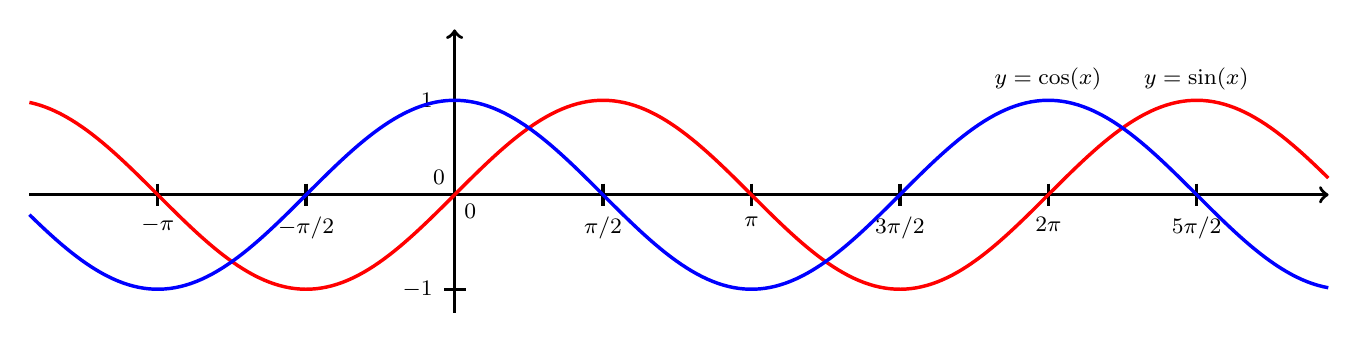
\begin{tikzpicture}[x=1.2cm,y=1.2cm]
		\draw[line width=1.25pt,->] (-4.5,0) -- (9.25,0) ;
		\draw[line width=1.25pt,->] (0,-1.25) -- (0,1.75) ;
		\draw (0,0) node[below right] {\footnotesize $0$} ;
		\draw (0,0) node[above left] {\footnotesize $0$} ;
		\foreach \y in {-1,1} \draw[line width=1.25pt] (4pt,\y) -- (-4pt,\y) node[left] {\footnotesize $\y$} ;
		\foreach \x/\val in {{-\pi}/{-pi},{-\pi/2}/{-0.5*pi},{\pi/2}/{0.5*pi},{\pi}/{pi},{3\pi/2}/{1.5*pi},{2\pi}/{2*pi},{5\pi/2}/{2.5*pi}} \draw[line width=1.25pt] (\val,4pt) -- (\val,-4pt) node[below] {\footnotesize $\x$} ;
		\draw[line width=1.25pt,red,samples=250,domain=-4.5:9.25] plot (\x,{sin(deg(\x))}) ;
		\draw[line width=1.25pt,blue,samples=250,domain=-4.5:9.25] plot (\x,{cos(deg(\x))}) ;
		\draw (6.28,1) node[above] {\footnotesize \blue $y=\cos(x)$} ;
		\draw (7.85,1) node[above] {\footnotesize \red $y=\sin(x)$} ;
	\end{tikzpicture}
\end{center}
Animation pour le tracé de la courbe de la fonction sinus : \url{https://www.geogebra.org/m/NQ9jcUVx}.
\end{cprop}

\end{document}